%----------------------------------------------------------------------------------
% Exemplo do uso da classe tcc.cls. Veja o arquivo .cls
% para mais detalhes e instruções.
%----------------------------------------------------------------------------------

% Seleção de idioma da monografia. Por enquanto as únicas opções
% suportadas são 'portuguese' e 'english'
% Para impressão em frente e verso, use a opção 'twoside'. Da
% mesma forma, use 'oneside' para impressão em um lado apenas.
\documentclass[portuguese,oneside]{UFFStex}
%\documentclass[english,oneside]{UFFStex}

%----------------------------------------------------------------
% Coloque seus pacotes abaixo.
%
% Obs.: muitos pacotes de uso comum do LaTeX, como amsmath,
% geometry e url já são automaticamente incluídos pela classe
% (veja o arquivo .cls). Isso torna obrigatória a presença destes
% no sistema para o uso desta classe, mas ao mesmo tempo o uso se
% torna mais simples.  Recomendo a instalação da versão mais
% recente da distribuição TeXLive (para Windows e UNIXes):
% www.tug.org/texlive/
%
% Pacotes e opções já incluídas automaticamente:
%
% \RequirePackage[T1]{fontenc}[2005/09/27]
% \RequirePackage[utf8x]{inputenc}[2008/03/30]
% \RequirePackage[english,brazil]{babel}[2008/07/06]
% \RequirePackage[a4paper]{geometry}[2010/09/12]
% \RequirePackage{textcomp}[2005/09/27]
% \RequirePackage{lmodern}[2009/10/30]
% \RequirePackage{indentfirst}[1995/11/23]
% \RequirePackage{setspace}[2000/12/01]
% \RequirePackage{textcase}[2004/10/07]
% \RequirePackage{float}[2001/11/08]
% \RequirePackage{amsmath}[2000/07/18]
% \RequirePackage{amssymb}[2009/06/22]
% \RequirePackage{amsfonts}[2009/06/22]
% \RequirePackage{url}
% \RequirePackage[table]{xcolor}[2007/01/21]
%\RequirePackage{lastpage}
%\RequirePackage{xparse}
%\RequirePackage{xstring}
%\RequirePackage{listofitems}
%----------------------------------------------------------------
% Para inserção de figuras.
\usepackage{graphicx}
\usepackage[table]{xcolor}
\definecolor{midgray}{gray}{.5}
% Utilize a opção 'pdftex' se você estiver usando o pdflatex (que
% permite figuras em formatos como .jpg ou .png)
%\usepackage[pdftex]{graphicx}

% Para tabelas com elementos ocupando mais de uma linha
\usepackage{multirow}
% Para frações na mesma linha (ex. ⅓).
\usepackage{nicefrac}
% Para inserir figuras lado a lado.
 \usepackage{subfigure}
% Para formatar algoritmos.
% A opção [algo2e] é necessária para evitar conflitos
% com as definições da classe.
% https://linorg.usp.br/CTAN/macros/latex/contrib/algorithm2e/doc/algorithm2e.pdf
\usepackage{algorithmic}
\usepackage[portuguese,algo2e,boxruled]{algorithm2e}
% Hyperlink em capitulos, seções, citações
\usepackage[hidelinks]{hyperref}	
% Bibliografia e citações padrão ABNT
%https://mirrors.ibiblio.org/CTAN/macros/latex/contrib/abntex2/doc/abntex2cite-alf.pdf
% Comandos: \citeonline{ref} \citeauthor{ref} \citeyear{ref}
%\usepackage[num]{abntex2cite}	% numérica
\usepackage[alf]{abntex2cite}	% alfabetica
% Referência cruzada que já coloca o tipo (Tabela, Figura, etc)
% a opção "brazilian" é para colocar em portugues (retirar a opção 
% quando escrever o texto em ingles/english
\usepackage[brazilian]{cleveref} 
% Pacote para revisão de texto
% alguns comandos de revisão:
% \alert{texto entre chaves}  \highlight{texto entre chaves}
% \remove{texto a ser removido} 
% \replace{texto original}{texto novo}
% \comment{texto original}{comentario adicionado}
% precisa ajustar a margem para evitar warning
\setlength {\marginparwidth }{2cm}
\usepackage{easyReview} 

%----------------------------------------------------------------
% Autor (OBRIGATÓRIO)
%----------------------------------------------------------------
\author{Allex Antoniollo}

%----------------------------------------------------------------
% Título (OBRIGATÓRIO). Devem ser passados DOIS parâmetros,
% o título em português E o inglês, não importando o idioma
% escolhido. Os títulos são utilizados para a montagem da capa,
% resumo e abstract mais tarde.
%----------------------------------------------------------------
\title{Segurança e Privacidade em Contratos Inteligentes: Desafios e Soluções no Ambiente Blockchain}
      {Security and Privacy in Smart Contracts: Challenges and Solutions in the Blockchain Environment}

%----------------------------------------------------------------
% Opções para o tipo de trabalho (OBRIGATÓRIO)
%----------------------------------------------------------------
\tipotrabalho{\tci}         % Trabalho de Conclusão I
%\tipotrabalho{\tcii}        % Trabalho de Conclusão II

%----------------------------------------------------------------
% Seleção do curso ("este trabalho é um requisito parcial para
% obtenção do grau de Bacharel em Ciência da Computação").
%----------------------------------------------------------------
\curso{\cc} % Ciência da Computação

%----------------------------------------------------------------
% Orientador (e Co-orientador, caso haja um). É OBRIGATÓRIO
% informar pelo menos o orientador.
%----------------------------------------------------------------
\orientador{EDIMAR ROQUE MARTELLO JUNIOR}
%\coorientador{Ciclano de Farias}

%----------------------------------------------------------------
% Palavras chave e Keywords
% Informar pelo menos 1 e no máximo 5 palavras chaves e Keywords,
%  separadas por virgula.
%----------------------------------------------------------------
\palavraschave{blockhain, contratos inteligentes,  vulnerabilidade, privacidade, segurança}
              {blochchain, smart contracts, vulnerability , privacy,  security}

%----------------------------------------------------------------
% A capa é inserida automaticamente. Por isso não é necessário
% chamar \maketitle
%----------------------------------------------------------------
\begin{document}

%----------------------------------------------------------------
% Ficha catalográfica (OBRIGATÓRIO para TCC II)
%  Você pode gerar a ficha neste link também: 
%   https://ficha.uffs.edu.br/
%----------------------------------------------------------------

%----------------------------------------------------------------
% Folha de aprovação (OBRIGATÓRIO para TCC II)
%   Primeiro parâmetro é a data da defesa
%   Demais parâmetros são os membros da banca (pelo menos 2 nomes)
%   Não precisa passar o nome do Orientador
%----------------------------------------------------------------

%----------------------------------------------------------------
% Depois da folha de aprovação vem a dedicatória e a epígrafe.
%----------------------------------------------------------------
\dedicatoria{Dedico este trabalho a meus pais.}

\epigrafe{The art of simplicity is a puzzle of complexity.}
         {Douglas Horton}

%----------------------------------------------------------------
% Também dá para fazer as duas na mesma página:
%----------------------------------------------------------------
%\dedigrafe{Dedico este trabalho a meus pais.}
%          {The art of simplicity is a puzzle of complexity.}
%          {Douglas Horton}

%----------------------------------------------------------------
% A seguir, a página de agradecimentos (OPCIONAL):
%----------------------------------------------------------------

%----------------------------------------------------------------
% Resumo (OBRIGATÓRIO)
%  As palavras chave são informadas no preambulo lá emcima (\palavraschave)
%----------------------------------------------------------------
\begin{resumo}
Este estudo concentra-se na análise crítica  de desafios de solução relacionados à segurança  e contratos inteligentes dentro do ecossistema blockchain.  
 Explorarei possíveis vulnerabilidades e ameaças à integridade  examinando casos de uso práticos.  
 A pesquisa tem como objetivo identificar  estratégias eficazes para riscos, destacando  melhores práticas tecnológicas que promovam a  implementação segura de inteligência.  
 Ao abordar esses tópicos, meu objetivo  é encontrar sugestões para uma compreensão mais profunda  e melhoria do no contexto de contratos inteligentes e  dos contratos inteligentes na blockchain.  
\end{resumo}

%----------------------------------------------------------------
% Abstract (OBRIGATÓRIO)
% %  As keywords são informadas no preambulo lá emcima (\palavraschave)
%----------------------------------------------------------------
\begin{abstract}
This study focuses on a critical analysis of challenges and solution strategies related to security and smart contracts within the blockchain ecosystem. I will explore potential vulnerabilities and threats to integrity by examining practical use cases. The research aims to identify effective strategies for risk mitigation, emphasizing technological best practices that foster secure implementation of smart contracts. By addressing these topics, my goal is to provide insights for a deeper understanding and improvement within the context of smart contracts and their implementation in the blockchain. 
\end{abstract}

%----------------------------------------------------------------
% Listas e sumário, nessa ordem. Somente o sumário é obrigatório,
% portanto, comente as outras listas, caso sejam desnecessárias.
%----------------------------------------------------------------
\listoffigures       % Lista de figuras      (OPCIONAL)
\listofacronyms      % Lista de siglas       (OPCIONAL)
\tableofcontents     % Sumário               (OBRIGATÓRIO)

%----------------------------------------------------------------
% Aqui começa o desenvolvimento do trabalho. Para uma melhor
% organização do documento, separe-o em arquivos,
% um para cada capítulo. Para isso, utilize o comando \include,
% como mostrado abaixo.
%----------------------------------------------------------------
%----------------------------------------------------------------------------------
% Exemplo do uso da classe tcc.cls. Veja o arquivo .cls
% para mais detalhes e instruções.
%----------------------------------------------------------------------------------
\chapter{Introdução}
\label{chap:intro}
% Comando para inserir siglas. As siglas devem aparecer em ordem ALFABÉTICA nas listas
% correspondentes. Como a classe no momento não é capaz de ordenar
% as entradas automaticamente, existem duas alternativas:
%
%    a- Insira todas as siglas no começo do texto,
%    manualmente e em ordem alfabética.
%
%    b- Caso esteja em um ambiente UNIX (Linux, Mac ou Cygwin/similares),
%    utilize o script sort.sh e o makefile que acompanham a
%    classe. O makefile automaticamente compila a monografia para
%    PDF (mas assume que o latex está acessível pela linha de
%    comando). Neste caso a ordenação é feita de forma automática.
%
\sigla{btc}{Bitcoin}
\sigla{BC}{Blockchain}
\sigla{SM}{Smart Contract}
\sigla{ZKP}{Zero-Knowledge Proof}
\sigla{DAAPS}{Aplicações Descentralizadas}
\sigla{DAOs}{Organizações Autônomas Descentralizadas}
\sigla{GGA}{Gas Griefing Attack}



%
%
% Comando para inserir símbolos. Estes irão aparecer em ordem
% de ocorrência, já que o número da página está presente na lista
% de símbolos.


\begin{itemize}
\item Introdução e Contextualização
	\begin{itemize}
 \item             Definição e Conceitos Básicos de Blockchain 
          \item História e Evolução da Tecnologia Blockchain
	   \item Princípios Fundamentais da Blockchain 
	   \item Smart Contracts: Fundamentos e Definições
	   \item Funcionamento e Aplicações Práticas

        \end{itemize}
\item Contratos Inteligentes e Privacidade: 
	\begin{itemize}
            \item Características dos Contratos Inteligentes
     \item Privacidade em Contratos Inteligentes 
        \end{itemize}
\item Riscos de Segurança em Contratos Inteligentes:
	\begin{itemize}	
            \item Ataques e Fraudes em Contratos Inteligentes
	    \item Exemplo de ataques bem sucedidos
     \item Vulnerabilidade Comum
     \item Gerenciamento de Risco em Smart Contracts
     \item Práticas Recomendadas para Mitigação de Risco

	\end{itemize}

\end{itemize}



\section{\label{sec:secao1}Definição e Conceitos Básicos de Blockchain}
A blockchain representa uma forma de estrutura de dados em cadeia, onde cada bloco recém-criado é incorporado à cadeia existente, aumentando assim o tamanho global da rede. Cada bloco contém dados e informações que estão intrinsecamente interligados, tornando qualquer tentativa de alteração ou exclusão de um bloco existente inviável, uma vez que tal modificação comprometeria a validação por toda a cadeia \cite{exame}.

Embora teoricamente exista a possibilidade de modificar informações dentro da blockchain, tal feito exigiria um poder computacional exorbitante em um intervalo de tempo incrivelmente curto. Esse desafio, por sua vez, torna-se uma tarefa não apenas complexa, mas também economicamente custosa de ser efetuada. À medida que mais blocos são adicionados à cadeia ao longo do tempo, a rede se expande, elevando consideravelmente o nível de complexidade. Isso resulta em uma barreira crescente para qualquer tentativa de influenciar a rede como um todo, conferindo à blockchain uma robustez e segurança notáveis.

A criptografia SHA-256, gera um hash com base, nas informações do bloco que acaba retornando um valor único por meio de uma operação criptografica. As funções hashs são muito utilizadas no quesito blockchain, a fim de adicionar segurança e imutabilidade \cite{bit2me}.


\subsection{História e Evolução da Tecnologia Blockchain}

Esta tecnologia teve sua origem na década de 90 como um banco de dados público e imutável. Somente em 1992, a criptografia foi incorporada ao seu funcionamento, elevando ainda mais a segurança e a integridade dos dados. No entanto, foi somente em 2008, com a criação do Bitcoin, que a blockchain encontrou seu primeiro uso prático e ganhou notoriedade como uma inovação revolucionária no campo da tecnologia da informação \cite{exame}.

Essa abordagem destaca a evolução da blockchain ao longo do tempo, enfatizando seus fundamentos iniciais, os aprimoramentos introduzidos com a criptografia e seu marco significativo com o advento do Bitcoin em 2008.


\subsection{Princípios Fundamentais da Blockchain}

\begin{itemize}
   \item Descentralização
   \item Consenso comum
   \item Trasnparência
    \item Segurança
   \item Imutabilidade
   \item Smart Contract
\end{itemize}

Descentralização implica na dispersão do poder central de uma autoridade, uma abordagem notável na tecnologia blockchain. Ao invés de concentrar todos os dados em um único servidor, a blockchain distribui essas informações entre os nós da rede, constituídos por diversos computadores que mantêm cópias sincronizadas da blockchain.

O consenso, elemento fundamental nesse contexto descentralizado, exige que qualquer informação passe por uma prova de concordância antes de ser adicionada à rede. Qualquer desvio em relação à expectativa impede a adição da informação, garantindo a integridade e confiabilidade do sistema.

A transparência é um princípio vital em blockchains públicas. Todas as transações e modificações são visíveis para todos os participantes da rede, estabelecendo um ambiente transparente que promove a confiança entre os usuários.

A segurança emerge como um catalisador fundamental para o crescente acolhimento da tecnologia, sendo a complexidade intrínseca dos algoritmos de hashing um fator preponderante. Atualmente, a violação destes algoritmos revela-se uma tarefa formidável, sobretudo diante da distância que os computadores quânticos modernos ainda necessitam percorrer para alcançarem tal proeza. Adicionalmente, a estratégia de reforçar a segurança por meio do aumento da quantidade de bits na criptografia se configura como uma abordagem eficaz para tornar esta missão ainda mais improvável.
Nesse contexto, propõe-se a transição do tradicional SHA-256 para o robusto SHA-512 como medida de fortalecimento da segurança \cite{Cointelegraph}.

A imutabilidade evita que os dados sejam modificados ou excluídos na rede.   
Esta característica resulta da combinação  do consenso coletivo de segurança criptográfica. 
Esta união cria uma base sólida  na qual a integridade dos dados é preservada com segurança.  
Imutabilidade, baseada no consenso  e segurança criptográfica, confiabilidade e inviolabilidade dos registros, constituindo assim  sistemas transparentes e segur

Os Smart Contracts, por sua vez, são como agentes autônomos na rede. São algoritmos programados para aguardar condições específicas antes de executarem suas funções. Ao serem implantados na rede, esses contratos inteligentes permanecem em estado de prontidão, sendo ativados automaticamente quando uma interação específica ocorre, desencadeando funcionalidades previamente programadas \cite{InfoMoney}.

\section{Smart Contracts: Fundamentos e Definições}

Os smart contracts são programas de computador autônomos e autoexecutáveis, incorporados em blockchain, que automatizam e garantem a execução de acordos sem a necessidade de uma autoridade central.
Esses contratos inteligentes são altamente versáteis e podem ser aplicados em diversas áreas. Embora seu uso seja mais evidente na transferência de valor, propriedade e informações, sua aplicabilidade vai muito além dessas funções essenciais.


\subsection{Origens e aplicações práticas}
O termo "smart contracts" foi cunhado por Nick Szabo em 1993. Szabo, um cientista da computação, propôs a ideia com o objetivo de introduzir práticas avançadas nos protocolos de comércio eletrônico entre indivíduos na internet, eliminando a necessidade de um intermediário central de confiança \cite{vector}. 

 A natureza programável e versátil dos smart contracts permite a implementação efetiva em uma variedade de cenários, incluindo jogos, votações, leilões, apostas, empréstimos e várias outras aplicações.

Atualmente, os smart contracts estão desempenhando um papel fundamental na transformação de setores, proporcionando eficiência, transparência e segurança. Sua capacidade de automatizar a execução de acordos, sem depender de intermediários, tem atraído atenção e adoção crescentes em várias indústrias.



\subsection{Desenvolvimento em Smart Contract}

Aplicações Descentralizadas (DAAPS) e Organizações Autônomas Descentralizadas (DAOs) são predominantemente aplicações baseadas na web que surgem do desenvolvimento de smart contracts. 

A imutabilidade da blockchain, que impede a alteração de dados uma vez registrados, representa uma característica fundamental desses contratos inteligentes. Isso significa que, uma vez implementado na blockchain, um smart contract não pode ser modificado, são . No entanto, existem métodos programáveis que possibilitam a atualização de smart contracts por meio de um mecanismo conhecido como "smart contract adapter"  \cite{atualizarSM}. Esse adaptador aponta para o endereço do smart contract que será utilizado, permitindo a extensão da mesma interface sem a necessidade de alterar diretamente o contrato existente.

Este processo de atualização proporciona flexibilidade e escalabilidade, pois permite que novas funcionalidades sejam incorporadas ou ajustes sejam feitos sem comprometer a integridade da blockchain. Essa abordagem de atualização programável, combinada com a natureza descentralizada das aplicações baseadas em blockchain, destaca a capacidade única desses sistemas de evoluir e se adaptar ao longo do tempo, sem depender de uma autoridade central. Isso reflete a inovação contínua no campo das tecnologias descentralizadas e ilustra como a combinação de contratos inteligentes e blockchain está moldando o futuro das aplicações na web.
%----------------------------------------------------------------------------------
% Exemplo do uso da classe tcc.cls. Veja o arquivo .cls
% para mais detalhes e instruções.
%----------------------------------------------------------------------------------
\chapter{\label{chap:chap2}Contratos Inteligentes e Privacidade}

Com base em  \cite{GGA}, a consideração sobre modificadores de acesso é frequentemente negligênciada por desenvolvedores de contratos inteligentes. Em contratos inteligentes, o encapsulamento não age como uma medida de segurança efetiva, dado que na blockchain, o acesso à informação é praticamente público para todos os participantes da rede. Embora os modificadores de acesso ajudem a organizar o código e a gerenciar o acesso entre contratos, é crucial compreender que, em blockchains públicas, a visibilidade das informações não é efetivamente controlada por esses modificadores.

O equívoco comum reside na crença de que marcar uma variável como privada a torna segura. No entanto, ao implantar um contrato na blockchain, esse código e todas as suas variáveis associadas são propagados por toda a rede. Isso significa que qualquer indivíduo que possua uma cópia do blockchain terá acesso às informações, independentemente do modificador de acesso.

Em decorrência disso, armazenar dados sigilosos ou delicados em variáveis privadas na blockchain é uma prática arriscada. Torna-se essencial adotar estratégias adicionais, como a criptografia e técnicas de ofuscação, para proteger informações sensíveis, reconhecendo que a simples marcação como "privado" não proporciona o nível de segurança desejado em um ambiente descentralizado e transparente como o das blockchains públicas.


\section{Característica dos Contratos Inteligentes}

Conforme discutido anteriormente, nos sistemas de blockchains públicas tradicionais, a natureza distribuída e pública dessas plataformas pode impactar a integridade e a privacidade dos dados. Essa consideração é relevante também neste contexto.

Em blockchains públicas, a visibilidade generalizada dos dados representa um desafio para a confidencialidade, pois qualquer pessoa pode acessar e verificar todas as transações registradas. No entanto, ao empregar tecnologias avançadas como a Zero-Knowledge Proof (Prova de Conhecimento Zero - ZKP), é possível mitigar esses desafios.

A implementação bem-sucedida de ZKP em sistemas blockchain públicos oferece uma solução eficaz para preservar a privacidade, permitindo que informações sensíveis permaneçam ocultas, mesmo em uma infraestrutura distribuída. Isso não apenas aprimora a segurança, mas também mantém a confiança dos usuários, promovendo a aceitação generalizada dessas plataformas.

 



\subsection{Desafios de Privacidade em Contratos Inteligentes}

\textbf{Prova de Conhecimento zero: }Com os avanços contínuos na tecnologia, a aplicação de ZKP tem se destacado como uma abordagem significativa para aprimorar a privacidade de dados durante transações em blockchain. A ZKP oferece a capacidade de preservar a confidencialidade de detalhes específicos, mesmo quando os dados da transação são registrados na blockchain.

Em ambientes descentralizados, como contratos inteligentes em decentralized applications (dApps), a implementação da prova de conhecimento zero emerge como uma medida crucial para fortalecer a segurança e atratividade dessas aplicações, especialmente aquelas que lidam com informações sensíveis. Ao incorporar ZKP nos contratos inteligentes, é possível assegurar que, mesmo quando os dados da transação são adicionados à blockchain, certos elementos permaneçam estritamente confidenciais.

Essa abordagem não apenas eleva os padrões de privacidade, mas também posiciona as dApps como soluções mais confiáveis para usuários preocupados com a segurança de seus dados. A capacidade de realizar transações sem divulgar informações específicas não apenas atende às demandas de privacidade, mas também impulsiona a confiança dos usuários em ambientes descentralizados \cite{SMPP}.

\textbf{Armazenamento em Banco de Dados: }De fato, a estratégia de armazenar dados sigilosos em um banco de dados, em vez de registrar tudo na blockchain, é uma abordagem alternativa que aborda preocupações de privacidade, mas ao custo da descentralização. Essa consideração também se aplica aqui.

Ao optar por um banco de dados centralizado para armazenar informações confidenciais, a descentralização inerente às blockchains é comprometida. A dependência de um servidor centralizado introduz um ponto único de falha e potenciais vulnerabilidades de segurança, pois um ataque ou falha nesse servidor pode comprometer todos os dados sensíveis.

Embora essa abordagem possa ser eficaz para proteger a privacidade dos dados, ela entra em conflito com os princípios fundamentais da descentralização que muitos sistemas blockchain visam alcançar. A centralização também implica maior controle e responsabilidade nas mãos da entidade que gerencia o servidor, o que pode gerar desconfiança por parte dos usuários.

Ao avaliar as opções entre descentralização e proteção de dados sigilosos, é fundamental encontrar um equilíbrio que atenda aos requisitos específicos da aplicação. 

 


\chapter{\label{chap:chap3}Riscos de Segurança em Contratos Inteligentes}


A presente seção visa fornecer uma análise aprofundada das diversas formas de ataque que podem ser direcionadas a smart contracts, destacando as vulnerabilidades que permeiam esse ecossistema complexo \cite{SMAP}. À medida que as implementações de contratos inteligentes se tornam uma peça fundamental em uma variedade de setores, compreender as possíveis brechas de segurança torna-se essencial para desenvolvedores, auditores e usuários. 

 Ao empregar smart contracts em uma blockchain, é imperativo reconhecer que uma vez implantados, esses contratos não podem ser atualizados ou modificados. Diante dessa imutabilidade, os patches de segurança da rede desempenham um papel crucial, servindo como uma salvaguarda vital contra potenciais vulnerabilidades.

Essa característica singular da blockchain impõe uma responsabilidade significativa sobre os desenvolvedores, incentivando-os a adotar uma estratégia de segurança robusta antes de lançar suas aplicações. Afinal, qualquer falha identificada após a implementação pode acarretar consequências potencialmente irreparáveis para o funcionamento da aplicação.


\section{Ataques e Fraudes em Contratos Inteligentes}

A crescente popularidade das aplicações de finanças descentralizadas (DeFi) na blockchain tem proporcionado um ambiente inovador para a criação e desenvolvimento de serviços financeiros autônomos. No entanto, à medida que novas plataformas DeFi são lançadas e atraem fundos de usuários, torna-se imperativo abordar os desafios significativos associados à segurança e proteção contra ataques. 


\subsection{Exemplo de ataques bem sucedidos}
Os dados foram obtidos em \cite{RA}.

\begin{itemize}


   \item \href{https://www.gemini.com/pt-br/cryptopedia/the-dao-hack-makerdao\#section-origins-of-the-dao}{The DAO Attack 2016 (\$60M)}
 
   \item \href{https://quillhashteam.medium.com/burgerswap-flash-loan-attack-analysis-888b1911daef}{BurgerSwap Attack 2021 (\$7.2M)}
 
   \item \href{https://www.zdnet.com/article/hackers-steal-25-million-worth-of-cryptocurrency-from-uniswap-and-lendf-me/}{Lendf.me Attack 2020 (\$25M)}
 
    \item \href{https://beosin.medium.com/a-sweet-blow-fb0a5e08657d}{XSurge Attack 2021 (\$4M)}
 
   \item\href{https://www.coindesk.com/business/2021/10/27/cream-finance-exploited-in-flash-loan-attack-worth-over-100m/}{Cream Finance Attack 2021 (\$18.8M)}
 
   \item \href{https://www.halborn.com/blog/post/explained-the-siren-protocol-hack-september-2021}{Siren Protocol Attack 2021 (\$3.5M)}


\end{itemize}

 
\subsection{Vulnerabilidades Comuns}

\textbf{Reentrancy Attack \cite{RA}: } Em um contexto de pesquisa acadêmica, é relevante destacar que na blockchain, os endereços de carteira e de smart contract têm a capacidade de receber e enviar criptomoedas. Isso permite a interação com smart contracts usando tanto uma carteira quanto outro smart contract. Este cenário é explorado por invasores, como descrito no exemplo a seguir, que visa elucidar um ataque de reentrancy.
\begin{figure}
    \centering
    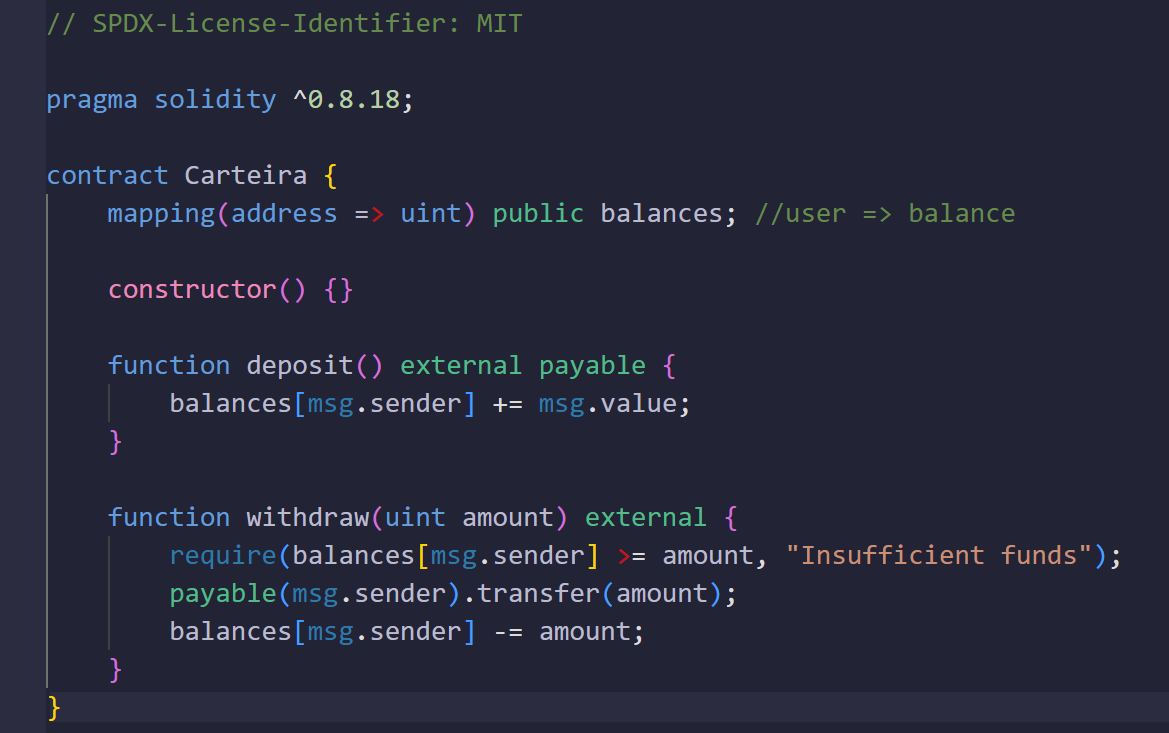
\includegraphics[width=0.5\linewidth]{figuras/VitimaRA.png}
    \caption{Contrato da Vítima}
    \label{fig:enter-label}
\end{figure}
\begin{figure}
    \centering
    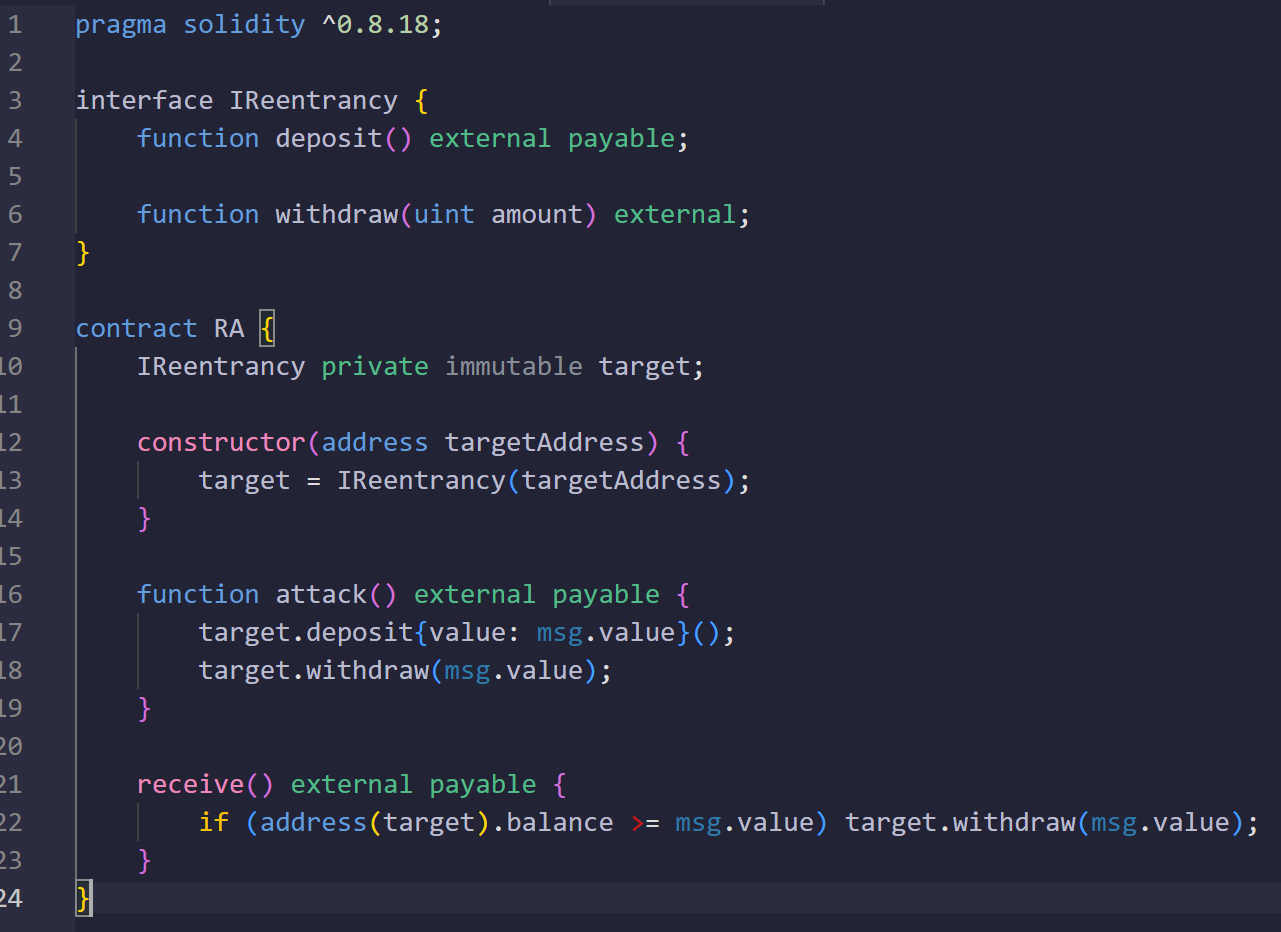
\includegraphics[width=0.5\linewidth]{figuras/RA.png}
    \caption{Contrato do Atacante}
    \label{fig:enter-label}
\end{figure}

Em um cenário hipotético, um invasor cria um smart contract, embora de forma mais sofisticada. O exemplo apresentado é simplificado, evitando a divulgação de ferramentas maliciosas. O contrato malicioso é então publicado na blockchain, identificando o endereço do contrato vulnerável.


Após o deploy do contrato malicioso, o atacante aciona a função "attack", realizando um depósito inicial no contrato alvo. Em seguida, ele invoca a função de saque do protocolo vítima, retirando a mesma quantidade recebida no depósito. Quando um smart contract recebe um saldo, a função nativa chamada "receive" é acionada. Embora, por padrão, essa função não execute ações, pode ser adaptada. No interior da função "receive", o invasor insere um código para realizar um novo saque, interrompendo a etapa de atualização do saldo do contrato vítima. Esse ajuste de balanço ocorre após o envio da transação, criando um loop até que o saldo do contrato seja exaurido. Em seguida, o invasor transfere o saldo final para outra conta, concluindo assim o ataque de reentrancy.

\textbf{Gas Griefing Attack \cite{GGA}:} Nos smart contracts de blockchain pública toda escrita é uma transação, e é exigido que toda transação pague uma taxa de gás -as taxas de gás sustentam a rede remunerando os validadores da rede-. 
Essa técnica consiste em fazer o contrato cobrar uma  taxa absurda ao ponto de zerar o saldo da carteira ou inviabilizar a lógica de negócio do contrato. 
Os contratos sucetiveis a esse ataque devem ser contratos que transferem dinheiro para outro endereço e disparam a função padrão receive, ou então em contratos que o atacante gostaria de interromper.
\begin{figure}
    \centering
    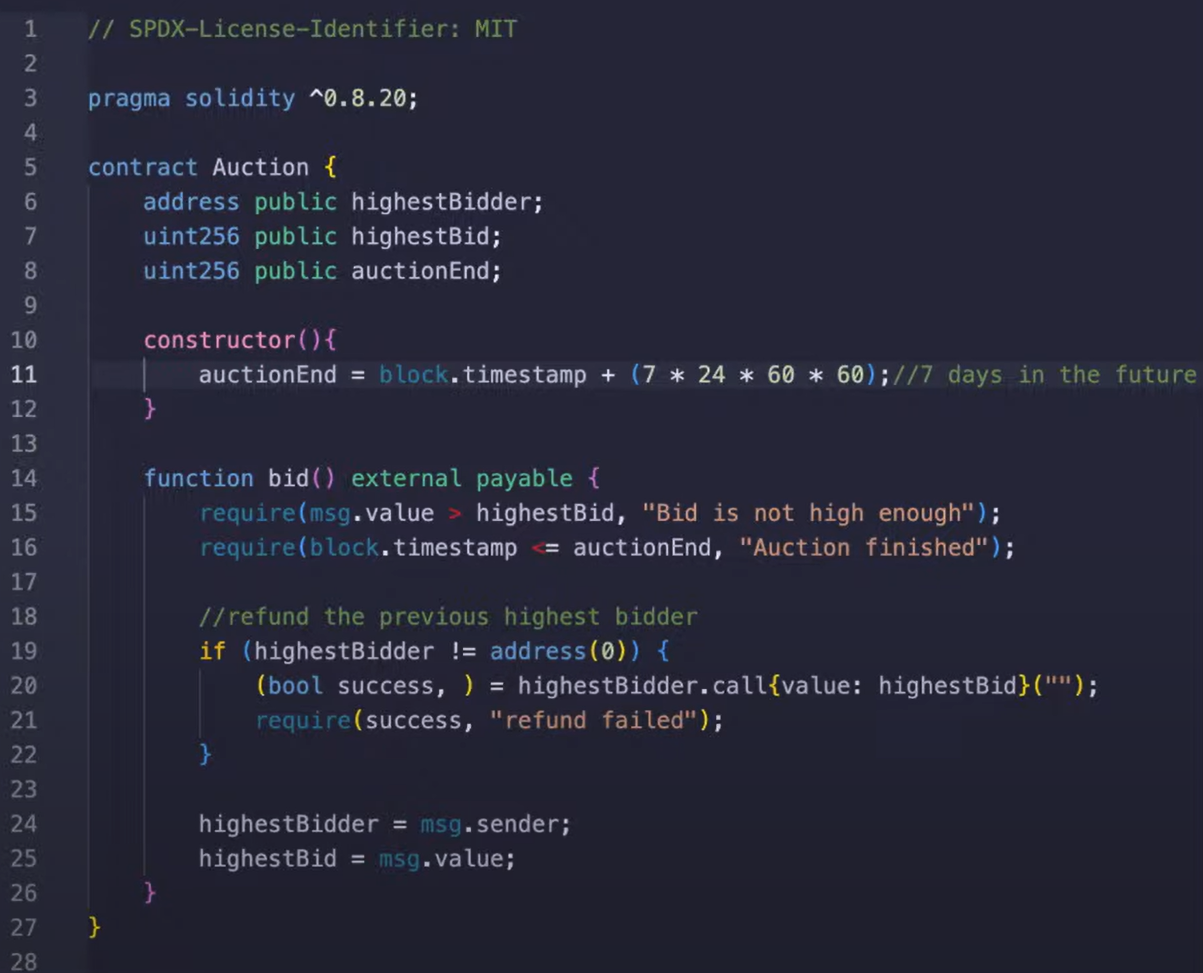
\includegraphics[width=0.5\linewidth]{figuras/Auction.png}
    \caption{Contrato de Leilão}
    \label{fig:enter-label}
\end{figure}

Este contrato de leilão foi concebido para operar ao longo de um período de 7 dias, apresentando uma função fundamental para dar lances. Quando um lance é submetido, o contrato realiza uma verificação para determinar se o novo lance supera o valor do lance máximo atual. Em caso afirmativo, ocorre uma atualização nas informações, resultando na alteração do vencedor do leilão para o usuário que ofereceu o novo lance. Além disso, os fundos são restituídos ao antigo vencedor do leilão.

Essa lógica de leilão busca promover a competição entre os participantes, garantindo que o usuário com o lance mais alto ocupe a posição de vencedor. A implementação de tal mecanismo proporciona dinamismo ao leilão, criando um ambiente em que os participantes podem ajustar seus lances para manter ou conquistar a liderança no decorrer dos 7 dias estabelecidos.

 \begin{figure}
    \centering
    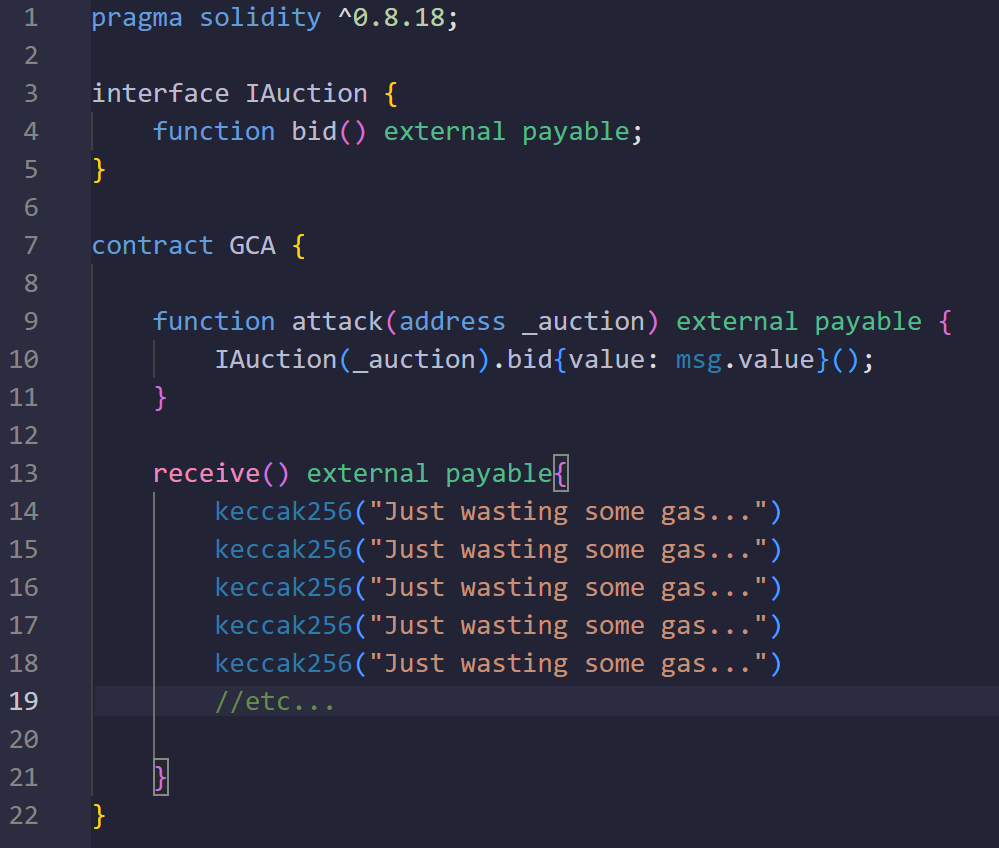
\includegraphics[width=0.5\linewidth]{figuras/GGA.png}
    \caption{Contrato do Atacante}
    \label{fig:enter-label}
\end{figure}

O contrato do atacante opera em consonância com o contrato do leilão, submetendo uma oferta superior à do atual líder. Quando outro participante oferece um lance superior ao do atacante, a função "receive" do contrato do atacante é invocada. Se o código presente em "receive"  for extenso ou complexo, isso pode acarretar em aumento das taxas devido à alocação de memória, podendo até ultrapassar o limite permitido para uma transação.

Quando um desses dois obstáculos ocorre, o contrato inteligente entra em um estado de erro, revertendo a transação original e mantendo o atacante como vencedor do leilão. Importante notar que o usuário que acionou a função enfrentará a perda de uma considerável quantia de gás da carteira, e em alguns casos, todo o valor destinado ao pagamento das taxas de transação.

Essa estratégia revela não apenas a manipulação do resultado do leilão pelo atacante, mas também destaca o potencial impacto financeiro adverso para quem efetuou a chamada da função. É crucial, portanto, que desenvolvedores e usuários estejam cientes dessas dinâmicas ao interagir com contratos inteligentes, priorizando a segurança e compreendendo as possíveis ramificações econômicas de suas ações na blockchain.

\section{Gerenciamento de Risco em Contratos Inteligentes}



\subsection{Práticas Recomendadas para Mitigação de Riscos}

\textbf{Reentrancy Attack \cite{RA}: }Sabendo a forma que um reentracy attack básico funciona, vamos ver duas principais observações que devem ser feitas para não cair em um ataque desse tipo.
\begin{figure}
    \centering
    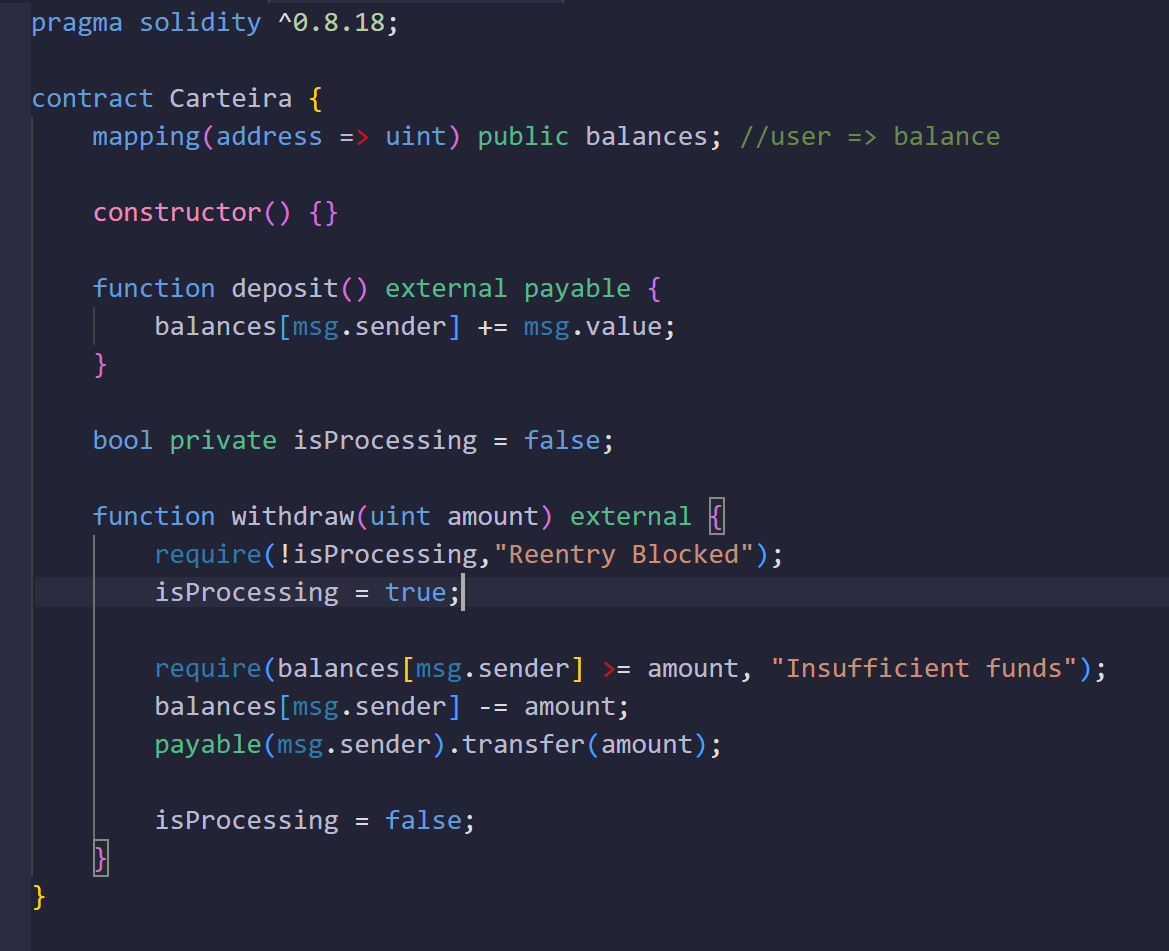
\includegraphics[width=0.5\linewidth]{figuras/RASolution.png}
    \caption{Solução Reentrancy}
    \label{fig:enter-label}
\end{figure}

É imperativo sempre manter a ordem das operações, dando prioridade à execução da atualização do saldo antes de qualquer transferência na função de saque. Ao organizar as etapas dessa maneira, evita-se a vulnerabilidade do código a ataques de reentrada com loops infinitos.

Outra medida eficaz para prevenir tais ataques na função de saque é a implementação de uma variável de controle dedicada. Essa abordagem, embora simples, proporciona uma camada adicional de segurança e pode ser aprimorada para uma implementação mais robusta. A lógica consiste em verificar e bloquear a possibilidade de reentrância na função de saque, impedindo potenciais explorações maliciosas.

Essas práticas, quando incorporadas, contribuem significativamente para mitigar a maioria dos ataques de reentrada, fortalecendo a segurança do protocolo.
\newline
\newline

\textbf{Gas Griefing Attack \cite{GGA}: } Diferentemente de alguns outros ataques a contratos inteligentes, esse tipo de ataque não possui uma solução simples, tornando-se assim uma ameaça significativa.

Em um cenário ideal, uma solução seria a atualização das linguagens de programação de contratos inteligentes para barrar sistemas como loops infinitos nas máquinas que executam os códigos.

Uma proposta mais radical seria alterar completamente o fluxo do contrato inteligente. Em vez de devolver imediatamente o dinheiro dos usuários quando alguém ultrapassa a oferta do atacante, o contrato poderia ser modificado para realizar a devolução apenas após o término do leilão. Essa alteração preservaria a integridade do contrato diante de ataques de GGA. No entanto, vale observar que uma mudança dessa natureza impactaria significativamente a lógica do contrato, exigindo adaptações no código para manter a equidade do leilão.

Por exemplo, se o dinheiro não fosse devolvido imediatamente quando alguém fizesse uma oferta maior, seria necessário implementar uma funcionalidade para permitir que o usuário com o dinheiro retido fizesse um novo lance utilizando os fundos bloqueados. Essas considerações destacam a complexidade de encontrar soluções eficazes que equilibrem a segurança do contrato com a manutenção da funcionalidade esperada.

\textbf{Os autores do artigo \cite{SMPP}} propõem a utilização da ferramenta "\href{https://github.com/eth-sri/securify2}{Securify}" como uma abordagem abrangente para identificar e compreender os problemas relacionados aos contratos inteligentes. Neste contexto, mais de 18 mil contratos inteligentes foram submetidos a testes, evidenciando a extensão e a diversidade do escopo de análise. A metodologia empregada pela "\href{https://github.com/eth-sri/securify2}{Securify}" permite a identificação de vulnerabilidades, destacando se os contratos inteligentes estão suscetíveis às formas mais básicas de ataques nesse domínio.

Essa abordagem não apenas oferece uma visão holística sobre a segurança dos contratos inteligentes, mas também fornece uma avaliação prática e abrangente da resistência desses contratos a ameaças potenciais. Ao realizar testes em uma quantidade significativa de contratos, os autores visam contribuir para uma compreensão mais profunda e generalizada dos desafios de segurança enfrentados pelos contratos inteligentes na blockchain.

 










 







\chapter{Cronograma}

O desenvolvimento deste trabalho se dará da seguinte forma:

\begin{enumerate}
    \item \label{ela-pro} Elaboração da proposta de TC.
    \item \label{anI} Estudo sobre o uso de dapps.
    \item \label{anII} Estudo sobre o uso de daos.
    \item \label{anIII} A implementação da tecnologia ZKP.
    \item \label{dI} Uso do Securify em SM.
    \item \label{dII} Aplicação de banco de dados em dapps e daos.
    \item \label{dIII} Sistema de versionamento de SM.
    \item \label{tec} Testes unitários e correções.
    \item \label{esc-tcII} Escrita do TC II.
\end{enumerate}

\begin{table}[!htbp]
    \centering
    \begin{tabular}{|c|c|c|c|c|c|c|c|c|c|c|}
        \hline
        &\multicolumn{5}{c|}{2023}&\multicolumn{5}{c|}{2024}\\
        \hline
        &MAR&ABR&MAI&JUN&JUL&AGO&SET&OUT&NOV&DEZ\\
        \hline
        \ref{ela-pro}&\cellcolor{midgray}&&&&&&&&&\\
        \hline
        \ref{anI}&&\cellcolor{midgray}&&&&&&&&\\
        \hline
        \ref{anII}&&\cellcolor{midgray}&&&&&&&&\\
        \hline
        \ref{anIII}&&\cellcolor{midgray}&\cellcolor{midgray}&&&&&&&\\
        \hline
        \ref{dI}&&&\cellcolor{midgray}&&&&&&&\\
        \hline
        \ref{dII}&&&\cellcolor{midgray}&\cellcolor{midgray}&&&&&&\\
        \hline
        \ref{dIII}&&&&\cellcolor{midgray}&\cellcolor{midgray}&&&&&\\
        \hline
        \ref{tec}&&&&&&&&\cellcolor{midgray}&\cellcolor{midgray}&\\
        \hline
        \ref{esc-tcII}&&&&&&&&\cellcolor{midgray}&\cellcolor{midgray}&\cellcolor{midgray}\\
        \hline
    \end{tabular}
\end{table}




%----------------------------------------------------------------
% Aqui vai a bibliografia. 
% Existem 2 estilos de citação definidos ao instanciar o 
% package abnt2tex: use
% 'alf' para citações do tipo [Abc+] ou [XYZ] (em ordem
% alfabética na bibliografia);
% 'num' para citações
% numéricas do tipo [1], [20], etc., em ordem de referência.
%----------------------------------------------------------------
\bibliography{bibliografia}


%----------------------------------------------------------------
% Após \appendix, se iniciam os capítulos de Apêndice, com
% numeração alfabética.
%----------------------------------------------------
%----------------------------------------------------------------
% Aqui vão os "capítulos" de anexos. Cada anexo deve
% ser considerado um capítulo.
%----------------------------------------------------------------
\anexos
\chapter{RAVitima.sol SM corrigido do ataque.}
\chapter{RA.sol SM do atacante de reentrancy}
\chapter{Auction.sol SM leilão atacado}
\chapter{GGA.sol SM do atacante de GGA}


\end{document}
